\documentclass[9pt,twocolumn,twoside]{gsajnl}
\newcommand{\sme}[1]{\textcolor{red}{\bf #1}}
\newcommand{\yang}[1]{\textcolor{orange}{\emph{\scriptsize  #1}} }
\graphicspath{{Figure_Table/}} \newcommand{\beginsupplement}{        \setcounter{table}{0}
        \renewcommand{\thetable}{S\arabic{table}}        \setcounter{figure}{0}
        \renewcommand{\thefigure}{S\arabic{figure}}     }

\articletype{inv} 
\newcommand{\X}{\textcolor{red}{\bf X\,}} \newcommand{\jri}[1]{\textcolor{blue}{ \emph{ #1}} } 
 \title{Deleterious genetic loads and their contributions to heterosis in genomic selection}  \author[$\ast$, 1]{Jinliang Yang} \author[$\ast$, 1, 2]{Sofiane Mezmouk} \author[$\dagger$]{Andy Baumgarten}
\author[$\ddagger$]{Rita H. Mumm}
\author[$\ast$, $\S$, 3]{Jeffrey Ross-Ibarra} 
\affil[$\ast$]{Department of Plant Sciences, University of California, Davis, CA 95616, USA}
\affil[$\S$]{Center for Population Biology and Genome Center, University of California, Davis, CA 95616, USA}
\affil[$\dagger$]{DuPont Pioneer, Johnston, IA 50131, USA}
\affil[$\ddagger$]{Department of Crop Sciences, University of Illinois at Urbana-Champaign, Urbana, IL 61801, USA}

\keywords{heterosis; deleterious; genomic selection; diallel; GERP; maize} 
\runningtitle{Genomic Selection Using GERP score} 
\correspondingauthor{Jeffrey Ross-Ibarra}

\begin{abstract}
Complementation of the deleterious alleles carried by the inbred parents may contribute to the vigorous performance, or heterosis, of the hybrid progenies. The detection of deleterious alleles was previous limited to the protein-coding regions. With the genomic evolutionary rate profiling (GERP), we extended the definition of deleterious alleles to the genome-wide. In total, about 86 million base-pairs, which make up 4.2\% of the maize genome, were detected as evolutionary conserved sequences in both genic and non-genic regions. Here we take advantage of evolutionary measures of sequence conservation to ask whether sites with prior evidence of functionality can inform GS models. We tested this idea using a partial diallel cross of 12 maize inbred lines. We sequenced the genomes of the parents and phenotyped both parents and hybrids for seven phenotypic traits across one environment in three years. We made use of an identity-by-decent analysis of the parents to identify haplotype blocks, and scored blocks in hybrids using a weighted sum of the GERP conservation score. We find that incorporating sequence conservation improves prediction accuracies in a five-fold cross-validation experiment for several traits \emph{per se} as well as heterosis for those traits. Because most variation at conserved sites is deleterious, we interpret these results as consistent with the simple complementation model for heterosis. Overall, this work demonstrates the importance of incorporating evolutionary information in GS and its potential usage in plant breeding.  \end{abstract}

\setboolean{displaycopyright}{true}
\RequirePackage[normalem]{ulem} \RequirePackage{color}\definecolor{RED}{rgb}{1,0,0}\definecolor{BLUE}{rgb}{0,0,1} \providecommand{\DIFadd}[1]{{\protect\color{blue}\uwave{#1}}} \providecommand{\DIFdel}[1]{{\protect\color{red}\sout{#1}}}                      \providecommand{\DIFaddbegin}{} \providecommand{\DIFaddend}{} \providecommand{\DIFdelbegin}{} \providecommand{\DIFdelend}{} \providecommand{\DIFaddFL}[1]{\DIFadd{#1}} \providecommand{\DIFdelFL}[1]{\DIFdel{#1}} \providecommand{\DIFaddbeginFL}{} \providecommand{\DIFaddendFL}{} \providecommand{\DIFdelbeginFL}{} \providecommand{\DIFdelendFL}{} 
\begin{document}

\maketitle
\thispagestyle{firststyle}
\marginmark
\firstpagefootnote
\correspondingauthoraffiliation{Department of Plant Sciences, University of California, Davis, CA 95616, USA. Email: rossibarra@ucdavis.edu}
\blfootnote{\textsuperscript{2}These authors contributed equally to this work}
\blfootnote{\textsuperscript{3}Current address: KWS SAAT AG, Grimsehlstr. 31, 37555 Einbeck, Germany}
\vspace{-11pt}





\lettrine[lines=2]{\color{color2}T}{}he phenomenon of heterosis has been observed across many species, from yeast \citep{Shapira2014} to vertebrates \citep{Gama2013}. Recent studies indicated that the complementation of the deleterious alleles, which fit classic dominant model, may play an important role in determining heterosis \citep{Charlesworth2009}. Deleterious alleles were arisen from new mutations during meiosis. In maize, about 90 new mutations were generated per meiosis \citep{Clark2005}, majority of which were deleterious according to empirical estimates \citep{Joseph2004}. In a natural outcross population, the negative effects on fitness of these deleterious alleles make them subject to be selection against, which lead the deleterious alleles to be maintained in a low frequency \citep{Eyre-Walker2007}. But the deleterious alleles could not be completerly purged. 

In maize, the total number of mildly deleterious mutations is substantial because of the exponential growth of population size after domestication. The modern breeding probably aims to remove these deleterious mutations and pyramiding beneficial alleles for agronomical purposes. In practice, the relatively homogeneous maize germplasm pool was artificially divided into different heterotic groups \citep{Heerwaarden2012}. It enabled the improvement of germplasm pools to be conducted in a parallel fashion, and therefore, facilitated the breeding efficiency. Using this hybrid breeding approach, the maize yield has been steadily improved since the early 20th century \citep{duvick2001biotechnology}. However, removing deleterious mutations in low recombination regions or in tightly linked regions become less effective. Studies indicated that residual heterozygosity correlates negatively with recombination \citep{Gore2009, McMullen2009} and the low recombination is effective over long period of time \citep{Haddrill2007}. As a consequence, the deleterious alleles would be accumulated in the low recombination regions, such as the pericentromeric regions in maize, and the vigorous performance could be realized by combining two sets of non-deleterious or beneficial alleles in repulsion state, thus lead to pesudo-overdominance. A recent QTL study identified loci controlling for heterosis are enriched in centromeric regions \citep{Lariepe2012}, which partly support this pesudo-overdominance hypothesis.

Despite the importance of deleterious alleles in contributing to heterosis, they have not been systematically investigated probably because of their low frequencies in the population and mostly exhibiting minor effects. Here, we employed a genomic selection (GS) approach to simultaneously estimate genome-wide deleterious variants in a half diallel population. The diallel population was composed of a set of hybrids, which enabled us to explore different modes of inheritance of the deleterious variants. And the study can be conducted with millions of variants but using relative little sequencing efforts. In our previous study, deleterious SNPs were found to be enriched in a SNP set identified by GWAS \citep{Mezmouk2014}. The deleterious variants in the study were defined as non-synonymous mutations in the coding regions. Clearly, deleterious variants are not limited to coding regions. Here, we expanded the characterization of deleterious variants to genome-wide using genomic evolutionary rate profiling (GERP) \citep{Cooper2005}. By incorporating GERP information in GS models, we demonstrated the prediction accuracies were significantly improved not only for some traits \emph{per se}, but aslo for some heterosis transformations (especially for traits exhibiting high levels of hereosis). Further studies indicated that joint effects of deleterious alleles with additive and dominant modes of inheritance may contribute to heterosis.


\section*{Materials and Methods} 

\subsection*{Plant material and phenotypic data}
\DIFdelbegin \DIFdel{Twelve }\DIFdelend \DIFaddbegin \DIFadd{We selected twelve }\DIFaddend maize inbred lines\DIFdelbegin \DIFdel{were selected and crossed in a half diallel fashion without considering reciprocal effects. Using this half diallel population , a field experiment was conducted in an incomplete block design with three replications. In the experiment, in addition to the }\DIFdelend \DIFaddbegin \DIFadd{, broadly representative of corn belt maize germplasm, as parents of a partial diallel population of }\DIFaddend 66 \DIFaddbegin \DIFadd{hybrids (each pair of parents crossed once) }\jri{i think figure S1 needs to show who was dad and mom for every hybrid. maybe just a table? needs to be cited here}\DIFadd{. We evaluated the }\DIFaddend F1 hybrids, \DIFdelbegin \DIFdel{the 12 }\DIFdelend inbred parents and two current commercial check hybrids \DIFdelbegin \DIFdel{were planted; and  hybrids and inbreds were grouped separately. The plants were grown at }\DIFdelend \DIFaddbegin \DIFadd{in the field in }\DIFaddend Urbana, IL \DIFdelbegin \DIFdel{in 2009, 2010 and 2011. }\DIFdelend \DIFaddbegin \DIFadd{over three years (2009-2011) in an incomplete block design. }\jri{were there 3 replicats each year? I was a bit confused}  \DIFaddend Plots consisted of four rows, with all observations taken from the inside two rows to minimize effects of shading and maturity differences from adjacent plots.  \DIFdelbegin \DIFdel{Both inbred lines and the 66 resulting hybrids were field evaluated. Phenotypic data was collected for }\DIFdelend \DIFaddbegin \DIFadd{We measured }\DIFaddend plant height (PHT, in cm), ear height (EHT, in cm), days to 50\% silking (DTS), days to 50\% pollen shed (DTP), anthesis-silking interval (ASI, in days), grain yield adjusted to 15.5\% moisture (adj GY, in bu/A), and test weight (TW, in pounds). \DIFaddbegin \jri{find out from Rita how to cite, distribute, phenotype data?}
\DIFaddend 

\DIFaddbegin \DIFadd{We estimated }\DIFaddend Best Linear Unbiased \DIFdelbegin \DIFdel{Estimation (BLUE}\DIFdelend \DIFaddbegin \DIFadd{Estimates (BLUEs}\DIFaddend ) of the genetic effects \DIFdelbegin \DIFdel{were calculated with }\DIFdelend \DIFaddbegin \DIFadd{in }\DIFaddend ASReml-R \citep{gilmour2009asreml} \DIFdelbegin \DIFdel{following the }\DIFdelend \DIFaddbegin \DIFadd{with the following }\DIFaddend linear model: 
\[Y_{ijkl} = \mu + \varsigma_{i} + \delta_{ij} + \beta_{jk} + \alpha_{l} +  \varsigma_{i} \cdot \alpha_{l} + \varepsilon\]
where 
$Y_{ijkl}$ is the phenotypic value of the $l^{th}$ genotype evaluated in the $k^{th}$ block of the $j^{th}$ replicate within the $i^{th}$ environment; 
$\mu$, the overall mean; 
$\varsigma_{i}$, the fixed effect of the $i^{th}$ environment;
$\delta_{ij}$, the fixed effect of the $j^{th}$ replicate nested in the $i^{th}$ environment; 
$\beta_{jk}$, the random effect of the $k^{th}$ block nested in the $j^{th}$ block; 
$\alpha_{l}$, the the fixed genetic effect  of the $l^{th}$ individual; 
$\varsigma_{i} \cdot \alpha_{l}$, the interaction effect of the $l^{th}$ individual with the $i^{th}$ environment; 
$\varepsilon$, the model residuals. \DIFaddbegin \jri{perhaps clarify "year" instead of "environment"?}
\DIFaddend 

\DIFdelbegin \DIFdel{Heterosis for each hybrid was then estimated by better-parental }\DIFdelend \DIFaddbegin \DIFadd{We estimated best-parent }\DIFaddend heterosis (BPH) \DIFaddbegin \DIFadd{as}\DIFaddend :
\[ BPH_{min,ij}=\hat{G_{ij}}-min(\hat{G_{i}} ,\hat{G_{j}}) \] 
\[ BPH_{max,ij}=\hat{G_{ij}}-max(\hat{G_{i}} ,\hat{G_{j}}) \]
where $\hat{G_{ij}}$, $\hat{G_{i}}$ and $\hat{G_{j}}$ are the genetic values of the hybrid and its two parents $i$ and $j$. $BPH_{min}$ was used instead of $BPH_{max}$ for days to anthesis. \DIFaddbegin \jri{what about ear height and DTS?}
\DIFaddend 

\subsection*{Sequencing and \DIFdelbegin \DIFdel{SNP calling}\DIFdelend \DIFaddbegin \DIFadd{Genotyping}\DIFaddend }

\DIFaddbegin \DIFadd{We extracted }\DIFaddend DNA from the twelve inbred lines \DIFdelbegin \DIFdel{was CTAB extracted \mbox{\citep{Doyle1987}
}and Covaris sheared for Illumina }\DIFdelend \DIFaddbegin \DIFadd{following \mbox{\citet{Doyle1987}
}and sheared the DNA on a Covaris }\jri{company, headquarters?} \DIFadd{for }\DIFaddend library preparation. \DIFdelbegin \DIFdel{The DNA libraries }\DIFdelend \DIFaddbegin \DIFadd{Libraries }\DIFaddend were then sequenced \DIFdelbegin \DIFdel{to an average coverage of 10X. 
}\DIFdelend \DIFaddbegin \jri{where? what length reads? insert size?}\DIFadd{. 
}\DIFaddend 

\DIFdelbegin \DIFdel{Raw paired reads (reverse and forward for each sequence), were trimmed }\DIFdelend \DIFaddbegin \DIFadd{We trimmed the raw sequenced data }\DIFaddend for adapter contamination with Scythe  \DIFdelbegin \DIFdel{package }\DIFdelend (\url{https://github.com/vsbuffalo/scythe}) \DIFdelbegin \DIFdel{which calculate the probability of having a contamination given the adapter sequence, the number of mismatches and sequence quality. The reads were then trimmed }\DIFdelend \DIFaddbegin \DIFadd{and }\DIFaddend for quality and sequence length ($\geq 20$ nucleotides) with Sickle \DIFdelbegin \DIFdel{package }\DIFdelend (\url{https://github.com/najoshi/sickle}). \DIFdelbegin 
\DIFdel{Read pairs, kept after filtering,  were mapped }\DIFdelend \DIFaddbegin \DIFadd{We mapped filtered reads }\DIFaddend to the maize B73 reference genome (AGPv2) with bwa-mem \citep{Li2009B}\DIFdelbegin \DIFdel{. Reads, }\DIFdelend \DIFaddbegin \DIFadd{, keeping reads }\DIFaddend with mapping quality (MAPQ) higher than 10 and with a best alignment score higher than the second best one \DIFdelbegin \DIFdel{, were kept }\DIFdelend for further analyses.
\DIFdelbegin 
\DIFdelend \DIFdelbegin \DIFdel{Single }\DIFdelend \DIFaddbegin \DIFadd{We called single }\DIFaddend nucleotide polymorphisms (SNPs) \DIFdelbegin \DIFdel{were called with }\DIFdelend \DIFaddbegin \DIFadd{using the }\DIFaddend $mpileup$ function from samtools utilities \citep{Li2009}. To deal with paralogy, which is a major problem in maize \DIFdelbegin \DIFdel{sequence mapping }\DIFdelend \citep{Chia2012}, all SNPs were filtered to a) be heterozygote in less than 3 inbred lines, b) have a mean minor allele depth over all genomes of at least 4, c) have a mean depth over all individuals lower than 30 and d) have missing/heterozygote alleles in less than 6 inbred lines (allelic information for at least 15 hybrids in the partial diallel design). 

\DIFdelbegin \subsection*{\DIFdel{Haplotype identification and SNP annotation}}

\DIFdelend \DIFdelbegin \DIFdel{All missing alleles were then imputed with BEAGLE package \mbox{\citep{Browning2009}
}and }\DIFdelend \DIFaddbegin \DIFadd{We used the fastIBD method implemented in BEAGLE \mbox{\citep{Browning2009,Browning2011}
}to impute missing data and identify regions of }\DIFaddend identity by descent (IBD) \DIFdelbegin \DIFdel{regions }\DIFdelend between the 12 inbred lines\DIFdelbegin \DIFdel{were identified with BEAGLE's fastIBD method \mbox{\citep{Browning2011}
}. The pairwise IBD region starts and ends were used to delimit haplotipic blocks where several inbred linesshared a homogenous haplotypes. }\DIFdelend \DIFaddbegin \DIFadd{. We then defined haplotype blocks as contiguous regions within which there were no IBD break points across all pairwise comparisons of the parental lines. }\jri{a supplemental figure here would help}
\DIFaddend 





\DIFaddbegin 


\subsection*{\DIFadd{Genomic selection using IBD blocks incorporated with GERP scores}}

\DIFaddend Genomic evolutionary rate profiling (GERP) \citep{Davydov2010}, which estimates the evolutionary constraint by quantifying substitution deficits after multiple genome alignments, was obtained from \citep{rodgers2015recombination} for AGPv2. 

\DIFdelbegin 
\subsection*{\DIFdel{Genomic selection using IBD blocks incorporated with GERP scores}}

\DIFdelend A haplotype based genomic selection (GS) strategy was conceived by using the IBD blocks as the explanatory variables, where the IBD blocks were coded with evolutionary conservation information. The reference genome sites with GERP score >0 were considered as conserved sites and genomic variants detected at these sites were determined as candidate deleterious alleles. To incorporate the conservation information into IBD blocks, SNPs falling into a given IBD block were added up using their estimated GERP scores. The sum of the score for a given IBD block were used as the conservation estimates of the IBD block. This estimation was calculated using a python script gerpIBD (\url{https://github.com/RILAB/pvpDiallel}) with both additive and dominant modes of inheritance. Under the additive model, 2 x GERP score was assigned to the homozygous loci with non-reference SNP calls; 1 x GERP score was assigned to the heterozygous loci; and 0 was assigned to the homozygous loci with reference SNP calls. Under the dominant model, 1 x GERP score was assigned to both the homozygous loci with non-reference SNP calls and heterozygous loci; 0 was assigned to homozygous loci with reference SNP calls.

To conduct prediction, a 5-fold cross-validation method was used, where the diallel population was randomly divided into training (80\%) and validation sets (20\%) for 10 times. The BayesC option in the GS software package of GenSel4 \citep{habier2011extension} was used for the model training, where 41,000 chains of iteration were used and the first 1000 chains were removed as a burn-in. After model training of the seven phenotypic traits \emph{per se} and their heterosis transformations, the prediction accuracies were obtained by comparing the predicted breeding values with the observed phenotypes in the corresponding validation sets. In addition, the GERP scores were circularly shuffled using 10-Mb window for 100 times as the null conservation estimates of the IBD blocks. Note that the cross-validation experiments using the circularly shuffled data were conducted on the same training and validation sets.  





\section*{Results}


\subsection*{Genetic values, heritability and heterosis transformations}

A half diallel population was created using 12 maize inbred lines (Figure \ref{fig:pvp-pheno}a). Two of them are important public inbreds, B73 and Mo17. And the other ten of them are proprietary inbreds (LH1, LH123HT, LH82, PH207, 4676A, PHG39, PHG47, PHG84, PHJ40, PHZ51) that have expired from Plant Variety Protection (PVP) and represent the lineage of key heterotic germplasm pools used in present-day commercial corn hybrids. The set is diverse enough to facilitate a broad sweep of the heterotic sub-groups that comprise U.S. commercial germplasm. From this population, phenotypic data were collected for seven traits of interest during 2009-2011. The phenotypic traits are anthesis-silking interval (ASI, in days), days to 50\% pollen shed (DTP), days to 50\% silking (DTS), ear height (EHT, in cm), grain yield adjusted to 15.5\% moisture (GY, in bu/A), plant height (PHT, in cm), and test weight (TW, in pounds).

The best linear unbiased estimators (BLUEs) for genotypes of the seven traits were derived from mixed linear models (Table S1). In the models, all fixed effects were significant (Wald test \emph{P} value < 0.05) for all traits except ASI for which the effect of the replicates within environments were not significant. As shown in the Figure \ref{fig:pvp-pheno}b, the BLUE values were normally distributed (normality test \emph{P} values > 0.05). The broad sense heritability of the traits ranged from 0.65 for ASI to 0.95 for PHT. With the parental phenotypic data, we conducted heterosis transformations using \DIFdelbegin \DIFdel{better-parental }\DIFdelend \DIFaddbegin \DIFadd{best-parent }\DIFaddend heterosis (BPH). Because the selected inbred lines are commercial relevant and fairly elite in performance, hybrids in this population exhibit relative low hybrid vigor (overall mean percent BPH = 0.3\% $\pm$ 0.4\%) normalized by their better parental data for most of the traits except GY (mean percent BPH = 95\% $\pm$ 16\%, Figure \ref{fig:pBPH}). Finally, general and specific combining ability (GCA ans SCA) were estimated following \citep{Falconer1996}. The GCA and SCA varied according to the traits (Table S2). For the GY, B73, PHG47 and PHG39 are the top three inbred lines that combining better with others.


\subsection*{Evolutionary constraint information for genomic variants}

In this study, all twelve inbreds were sequenced to an average depth of $\sim$10X. Reads were mapped to the maize B73 reference genome (AGPv2) with bwa-mem. After filtering of depth, heterozygosity and missingness, 13.8 million SNPs were kept, including 1.9 million SNPs in genic regions and 361,280 in protein coding regions. We estimated the allelic error rate by first comparing our genotype calls to those of 41,292 overlapping SNPs on the maize SNP50 bead chip \citep{Heerwaarden2012}; and then compared our SNP alleles for B73 and Mo17 with the 10,426,715 SNP previously identified in HapMap2 \citep{Chia2012}; finally, we compared our SNPs to 180,313 overlapping SNPs identified through genotyping by sequencing (GBS) \citep{Romay2013}. The comparisons showed 99.12\% allele similarity with shared SNPs previously identified.  

Evolutionary constraint information of GERP was obtained from \citep{rodgers2015recombination}, which was computed by using rejected substitution rate relative to the neutral rate after multiple genome squences alignment \citep{Davydov2010}. This approach could estimate the conservation information at the base-pair level, extending the definition of deleterious variants to non-genic regions compared to previous approaches of SIFT \citep{ng2003sift} or MAPP \citep{stone2005physicochemical}. In AGPv2, more than 86 million bases ($\sim$4.2\% of the maize genome) were detected as evolutionary constraint bases with GERP score >0. From genome-wide of view, genomic sequences are evolutionarily constraint near the telomeric regions and the mean GERP scores dropped, in general, toward centromeric regions (Figure \ref{fig:dis1m}) with some exceptions at long arm of chromosome 1 and 4.  

Although genomic sites with GERP score >0 showed evidence of under evolutionary constraint, they are not immune to mutate. Indeed, in our diallel population, 506,898 SNP variants were detected at sites where the GERP scores are bigger than zero (Figure \ref{fig:gerpmaf}A). Consistent with previous study \citep{rodgers2015recombination}, the minor allele frequencies (MAFs) of these SNPs were negatively correlated with their GERP scores (Pearson's correlation test \emph{P} value < 0.05, \emph{r} = $-0.8$), indicating that the putative deleterious alleles tend to be purged and maintained in a low frequency in the population. 


\begin{figure}[htbp]
\centering
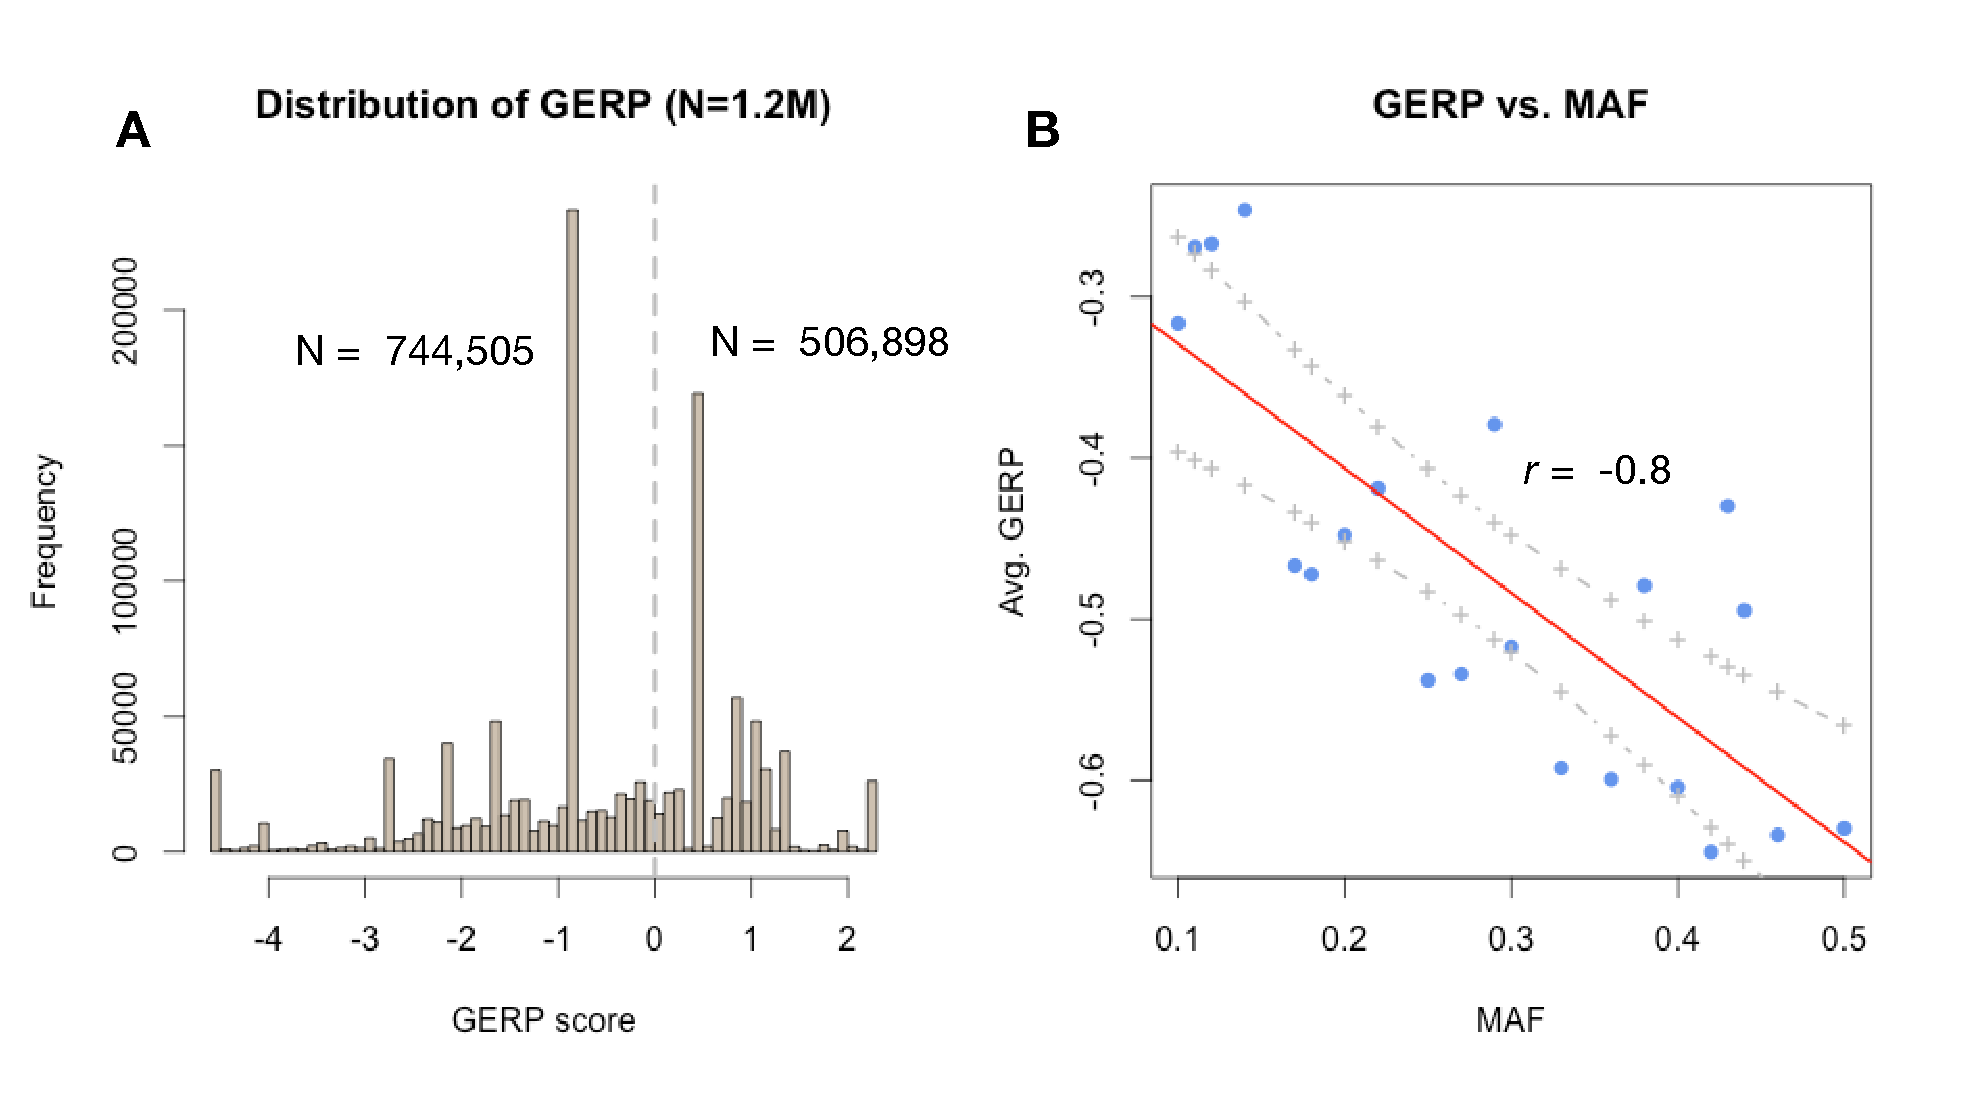
\includegraphics[width=\linewidth]{Figure_gerpmaf.pdf}
\caption{Distribution of GERP scores and relationship between GERP scores and MAFs. \textbf{(A)} GERP scores were extracted for $\sim$1.2 million SNPs ($\sim$10\% of the total SNPs) of the diallel population. The spikes in the histogram were because only limited genomes (N < 10? \yang{ask for this number}) were used in GERP calculation. \textbf{(B)} Mean GERP scores were calculated for each bin (bin size = 0.01) of minor allele frequency (MAF). The red line and grey lines define the regression and its 95\% confidence interval.}
\label{fig:gerpmaf}
\end{figure}


\subsection*{Incorporatipn of GERP information improved prediction accuracies}

Genomic variants occurred at the evolutionary constraint sites were potentially deleterious. The phenotypic effects of these genetic loads and their contributions to heterosis become an interesting area to explore. However, the population size in this study is relative small and SNPs detected at sites containing high GERP scores are generally in low frequencies. The statistical power to detect the separate effects of these putative deleterious alleles becomes very low. To alleviate the statistical limitations, we conceived a haplotype-based approach for GS, which could add up individual effects of deleterious alleles in IBD blocks and estimate these IBD blocks simultaneously. To conduct the analysis, first of all, 55,000 IBD blocks were identified, which had an average size of 44,980 bp (ranged from 36 to 10,320,000 bp). IBD blocks having > 1-kb in size and containing > 1 deleterious alleles (SNPs at sites with GERP scores >0) were kept for further analysis. Secondly, the GERP scores of SNPs in an IBD block were summed under both additive and dominant models. Those summed GERP scores on IBD blocks were considered as the measurements of the conservation of the haplotypes. More details of this procedure were illustrated in Figure \ref{fig:gerpibd}.      

A Bayesian-based statistical method (BayesC) \citep{habier2011extension} was employed for model training. Using a 5-fold cross-validation approach, the prediction accuracies of the real data and cicularly shuffled data were compared. As shown in Figure \ref{fig:gerpall}, for traits \emph{per se}, prediction accuracies were significantly (FDR < 0.05) improved for ASI and PHT when incorporating GERP information in the IBD blocks under the additive model; prediction accuracy was significantly improved for ASI under the dominant model. For heterosis transformation traits (BPH), incorporation of GERP scores improved BPH of GY under the additive model and improved BPH of DTP, DTS and TW under the dominant model (Figure \ref{fig:gerpall} C and D, Supplementary table 3). In general, the average prediction accuracis were higher using the additive model (mean \emph{r} = 0.81 and 0.49 for traits \emph{per se} and BPH) than the dominant model (mean \emph{r} = 0.70 and 0.42). And the prediction accuracies decreased for predicting heterosis transformations (BPH) as compared to the predictions for traits \emph{per se}.

It was argued that SNPs in genic regions might have higher GERP scores than those in non-genic regions. The circular shuffling permutations may shift the high GERP scores to non-genic regions. If that is the case, the approach tended to weigh more on genic SNPs. To rule out this possibility, we elected SNPs with GERP scores >0 in genic regions only and did the circular shuffling to assign GERP scores to the same set of the selected SNPs. By doing this, the method will not take advantage of genomic positional information any more. Noted that in this study less number of SNPs was selected (N = 316, 983). Nevertheless, model prediction accuracies were significantly improved for traits \emph{per se} of GY under the additive model. For heterosis transformations, prediction accuracies were significantly improved for BPH of GY and PHT under the additive model and the prediction accuracy was significantly improved for pBPH of GY (Figure \ref{fig:genicsnp} and Table S4).   


\begin{figure}[htbp]
\centering
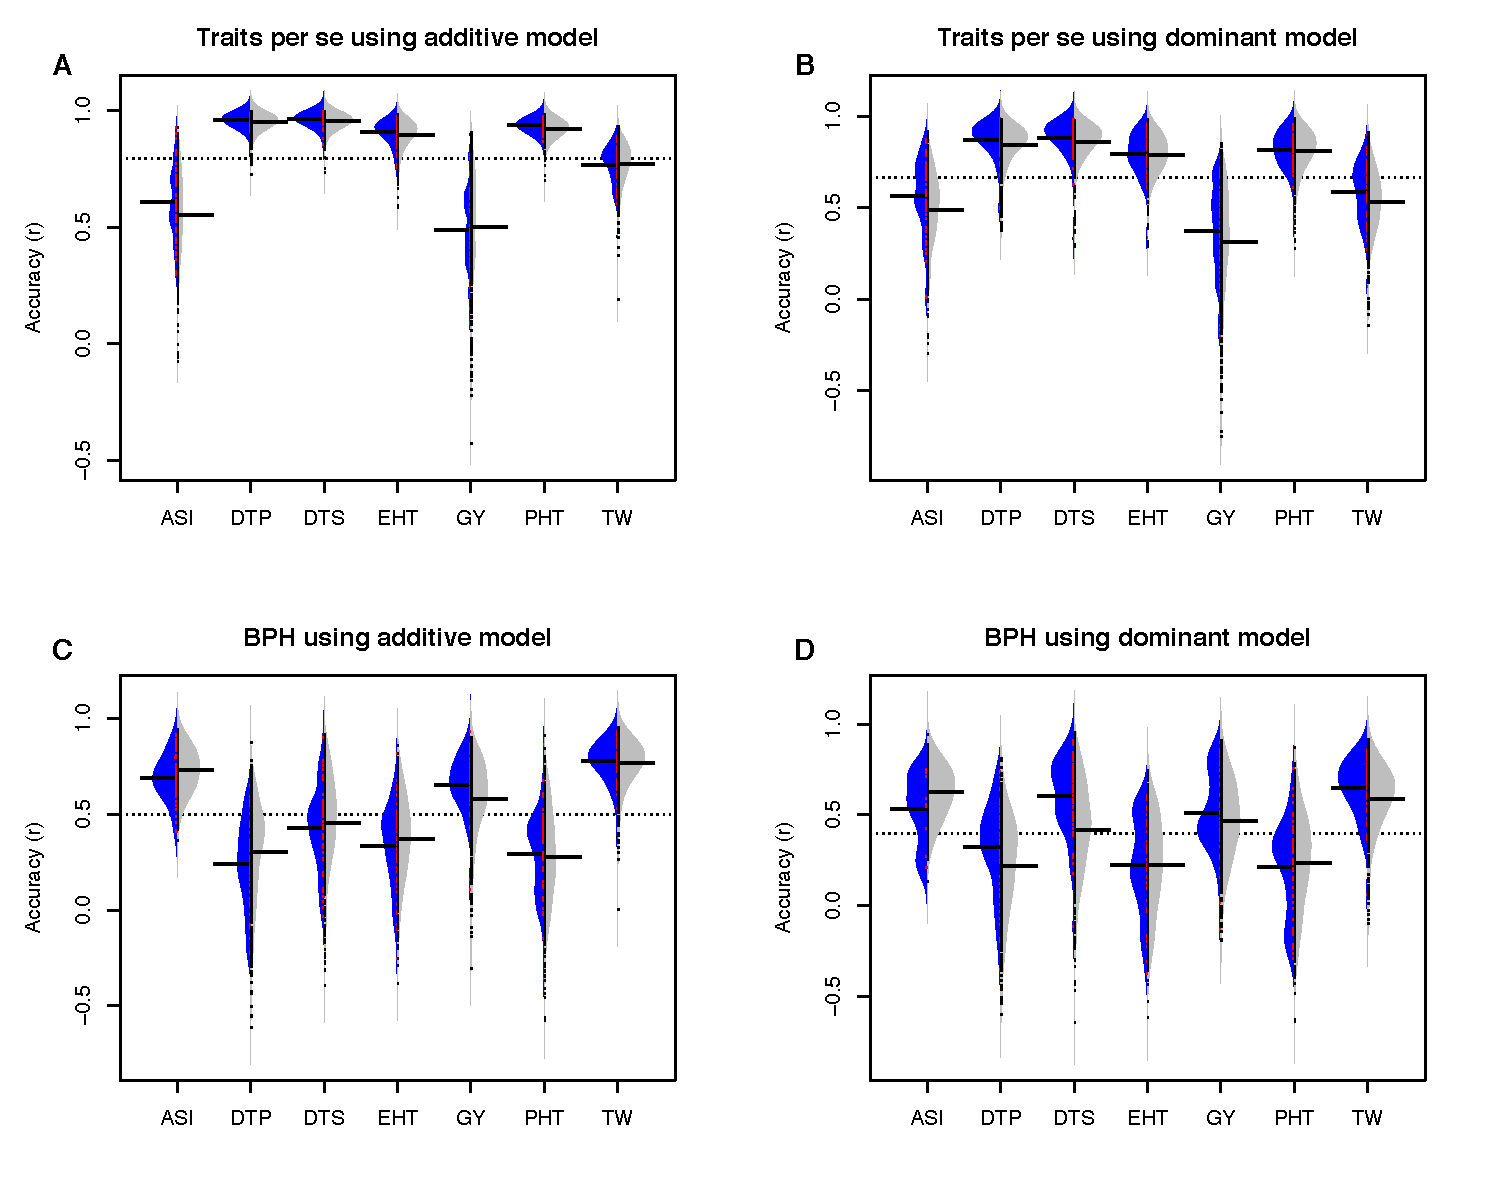
\includegraphics[width=\linewidth]{Figure_gerpall.pdf}
\caption{Beanplots of cross-validation accuracies using SNPs with positive GERP score. Cross-validation experiments were conducted using selected SNPs and circular shuffled data from the same set of SNPs for traits \emph{per se} (\textbf{A, B}), HPH (\textbf{C, D}) and pHPH (\textbf{E, F}) under additive (\textbf{A, C, E}) and dominant (\textbf{B, D, F}) models. Accuraries from the real data were plotted on the left side of the bean (blue) and permutation results plotted on the right (grey). Horizotal bars on beans indicate mean accuracies. The grey dashed lines indicate the overall average accuracies. Stars indicate significantly improved cross-validation accuracies with FDR < 0.05.}
\label{fig:gerpall}
\end{figure}


\subsection*{Posterior phenotypic variance explained and model comparisons}

To learn why the prediction performace varied among traits \emph{per se} and heterosis transformations, we obtained the posterior variance explained by our models using the complete set of data. As shown in Figure \ref{fig:h2}, additive models explained more phenotypic variance for traits \emph{per se} of DTP, DTS, EHT and PHT; but explained less phenotypic variance for heterosis transformations (BPH) of ASI, GY and TW. On the contrary, lager proportions of the phenotypic variance could be explained by the dominant models for heterosis transformations (BPH) of ASI, GY and TW. For the GY in particular, 50\% of the heterosis could be explained by dominant model.   

Heterosis transformations were largely determined by the accuracies of the parental phenotypes. To take the uncertainty of the parental phenotypes into consideration, we estimated the combining abilities from the hybrid population itself to investigate which modes of inheritance perform better than the null models. We extracted the breeding values estimated with both additive and dominant models using the genome-wide IBD blocks incorporated with the GERP scores. Consistent with above analysis, IBD blocks coded with dominant mode of inheritance significantly (equation \ref{eq:refname1} vs. equation \ref{eq:refname2}, ANOVA \emph{P} value < 0.05 ) improved model fitting for ASI and GY. We also compared model \ref{eq:refname3} and model \ref{eq:refname4}, ANOVA results indicated that \ref{eq:refname4} performed almost as good as \ref{eq:refname3}, indicating that specific combining ability captured most of the parental interactions and the current method could not detect higher order of interactions. 

\begin{equation}
Y_{ij} = \mu + GCA_{i} + GCA_{j} + \varepsilon
\label{eq:refname1}
\end{equation}
\begin{equation}
Y_{ij} = \mu + GCA_{i} + GCA_{j} +  G_{ij} + \varepsilon
\label{eq:refname2}
\end{equation}
\begin{equation}
Y_{ij} = \mu + GCA_{i} + GCA_{j} + SCA_{ij} + \varepsilon
\label{eq:refname3}
\end{equation}
\begin{equation}
Y_{ij} = \mu + GCA_{i} + GCA_{j} + SCA_{ij} + G_{ij} + \varepsilon
\label{eq:refname4}
\end{equation}
where 
$Y_{ij}$ is the BLUE value of the hybrid crossed between the $i^{th}$ inbred and $j^{th}$ inbred; 
$\mu$, the overall mean; 
$GCA_{i}$, the general combining ability of the $i^{th}$ inbred;
$GCA_{j}$, the general combining ability of the $j^{th}$ inbred;
$SCA_{ij}$, the specific combining ability of between the $i^{th}$ and $j^{th}$ inbreds;
$\varepsilon$, the model residuals.

\begin{figure}[htbp]
\centering
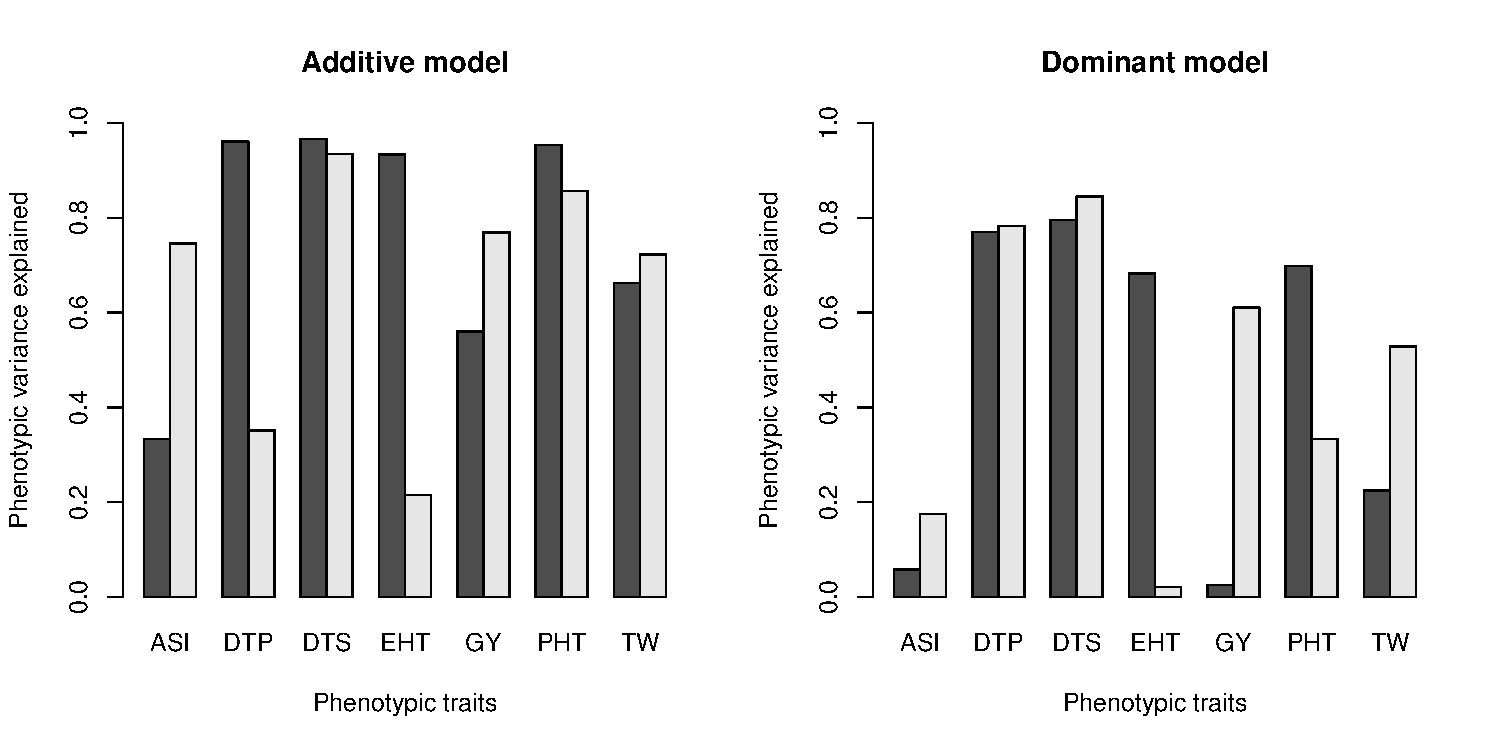
\includegraphics[width=\linewidth]{Figure_h2.pdf}
\caption{Barplots of the phenotypic variance explained by IBD blocks incorporated with GERP scores.}
\label{fig:h2}
\end{figure}


\section*{Discussion}

\begin{itemize}
  \item how do results match with heritability and heterosis?
  \item do we support deleterious model of Mezmouk et al.?
\end{itemize}


In this study, more than 500,000 deleterious SNPs were identified in elite maize lines including in non-coding regions of the genome. Majority of them were maintained in a low frequency, which consistent with the previous observation \yang{Eli PNAS, 2015} and indicated the deleteriousness of the variants in the conserved sites. To estimate the joint effects of the potentical deleterious alleles for the phenotype, a genomic selection pipeline was developed, which utilized evolutionary conservation information in the IBD blocks as explainatroy variables. After model training, cross-validation results suggested prediction accuracies for some traits \emph{per se} and heterosis transformations could be significantly improved by incorporating GERP scores. 

Paritcally, with dominant model, up to 20\% of the phenotypic variance could be explained for the heterosis traits. Theoritically, BPH transformation subtracts the joint effects of the additive and dominant alleles in the best parents as residule, the substantiall variance of these redidules explained by the additive or dominant models in our studies indicated that genetic components controlling for heterosis might in linked state. Note that the current model simply assume the traits were simply determined by complete additive or complete dominant. In the real case, the phenotype most likely be controlled by some degree of mixture of additive and dominant complenents. 

Schmitt: How to explain the prediction difference?  
The variation of the prediction accuacies were relative large in this study. First of all, broad sense heritability of the traits are different. Second, from the simulation we learned that different traits may controlled by different proportion of additive, dominant and even recessive gene actions. Our naive model only built the pure additive and pure dominant effects in. For the more complicated cases, the models may not work very well.

\clearpage
\bibliography{Diallel}


\pagebreak
\beginsupplement
\section*{Supporting Information}

\DIFaddbegin \onecolumn
\DIFaddend \begin{center}\vspace{1cm}
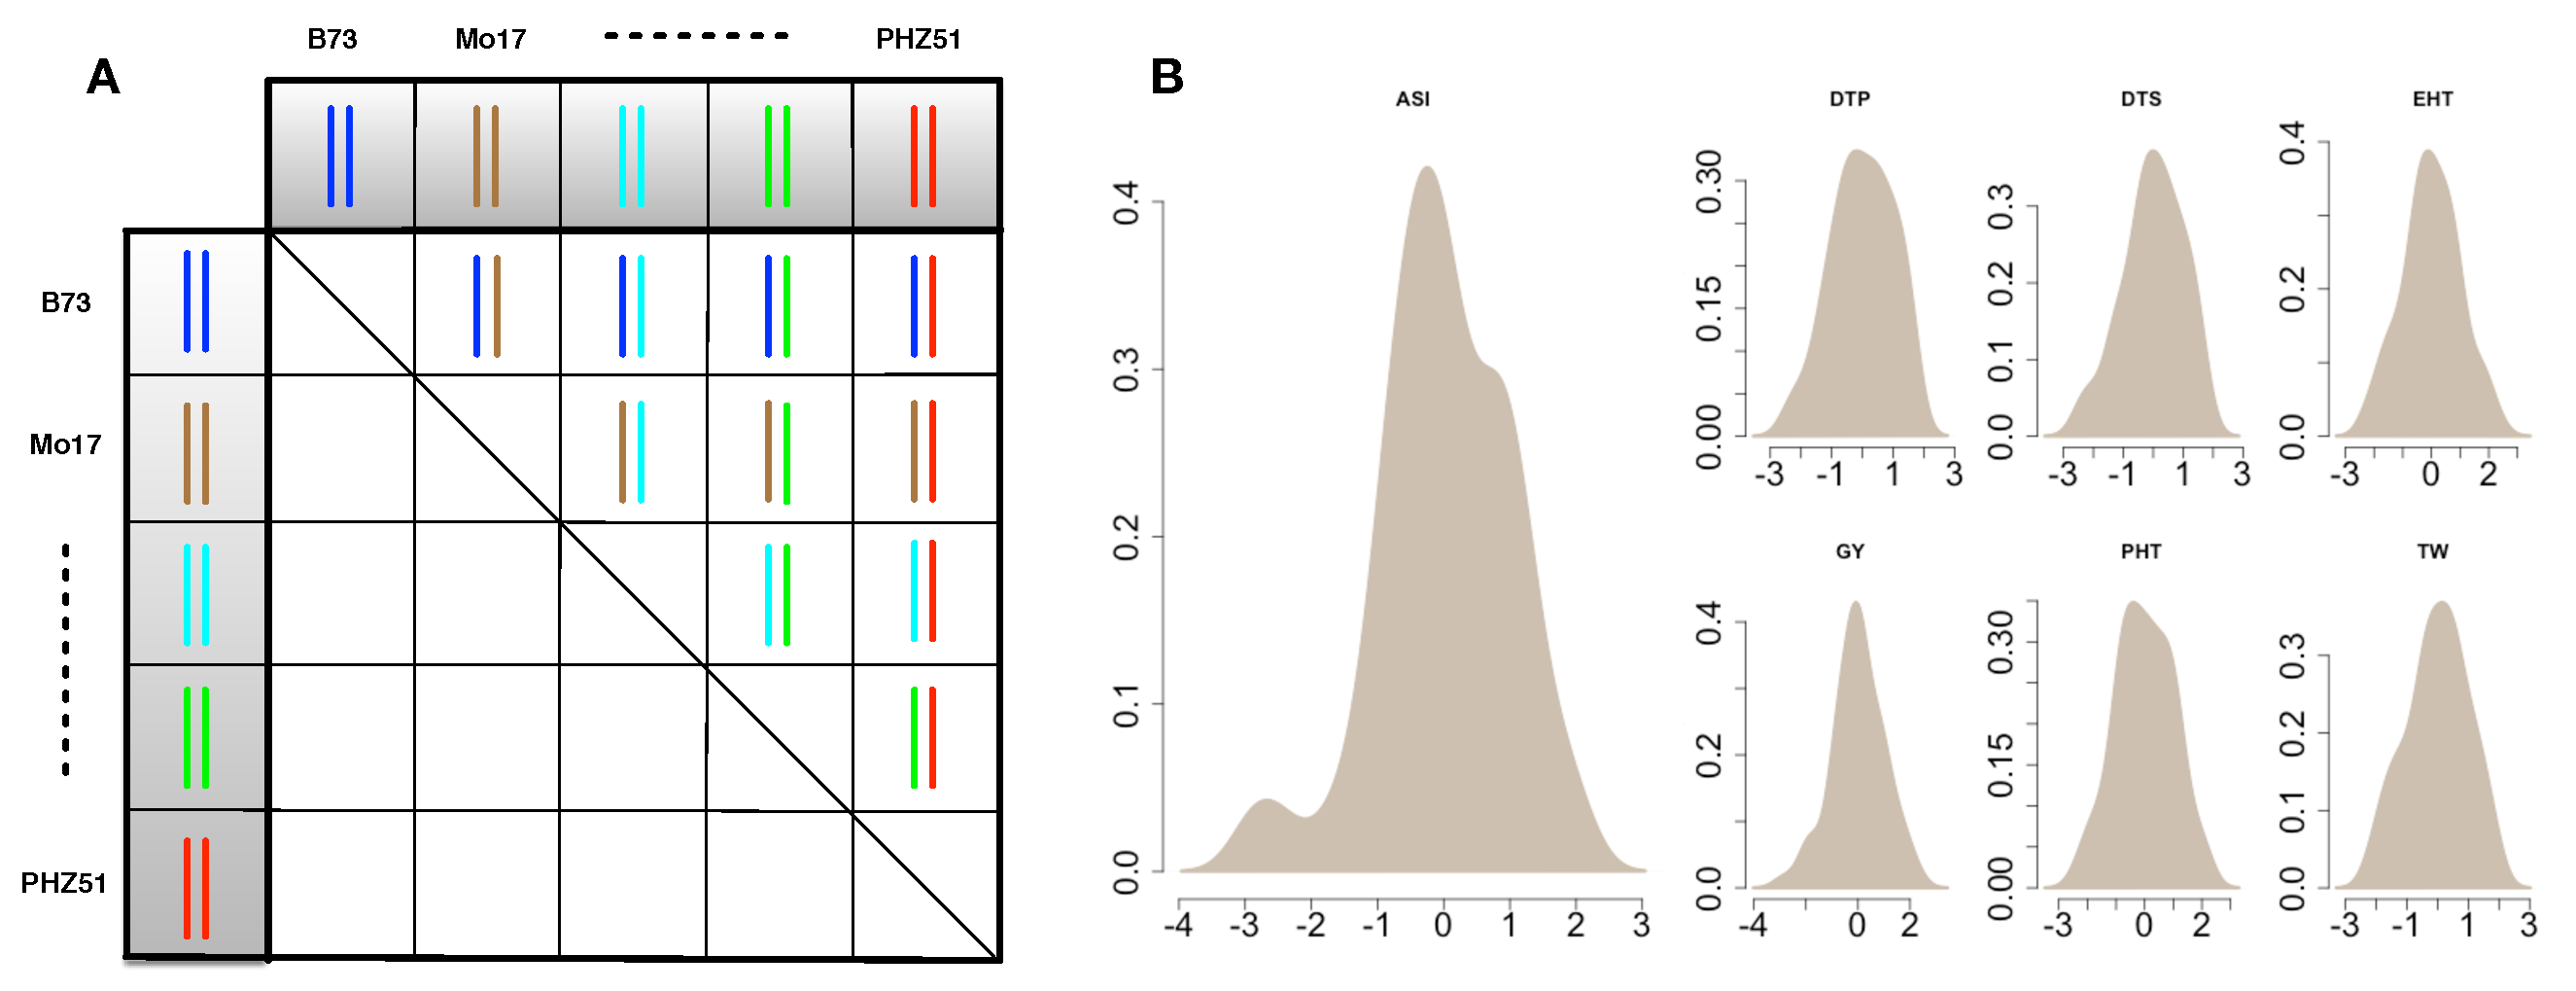
\includegraphics[width=0.8\linewidth]{SFig_pvp.pdf}
\captionof{figure}
{\color{black} \textbf{Diallel experimental design and distribution of phenotypic data.}
\textbf{(A)} Twelve maize inbred lines were selected and crossed in a half diallel. \textbf{(B)} Density plots of the phenotypic distributions.
}
\label{fig:pvp-pheno}
\end{center}\vspace{1cm}

\begin{figure}[htbp]
\centering
\includegraphics[width=\linewidth]{SFig_pBPH.pdf}
\caption{Boxplot of the percent better parental heterosis (pBPH). In the plot, ASI was calculated using pBPHmin and the other six traits were calculated using pBPHmax.}
\label{fig:pBPH}
\end{figure}

\begin{figure}[htbp]
\centering
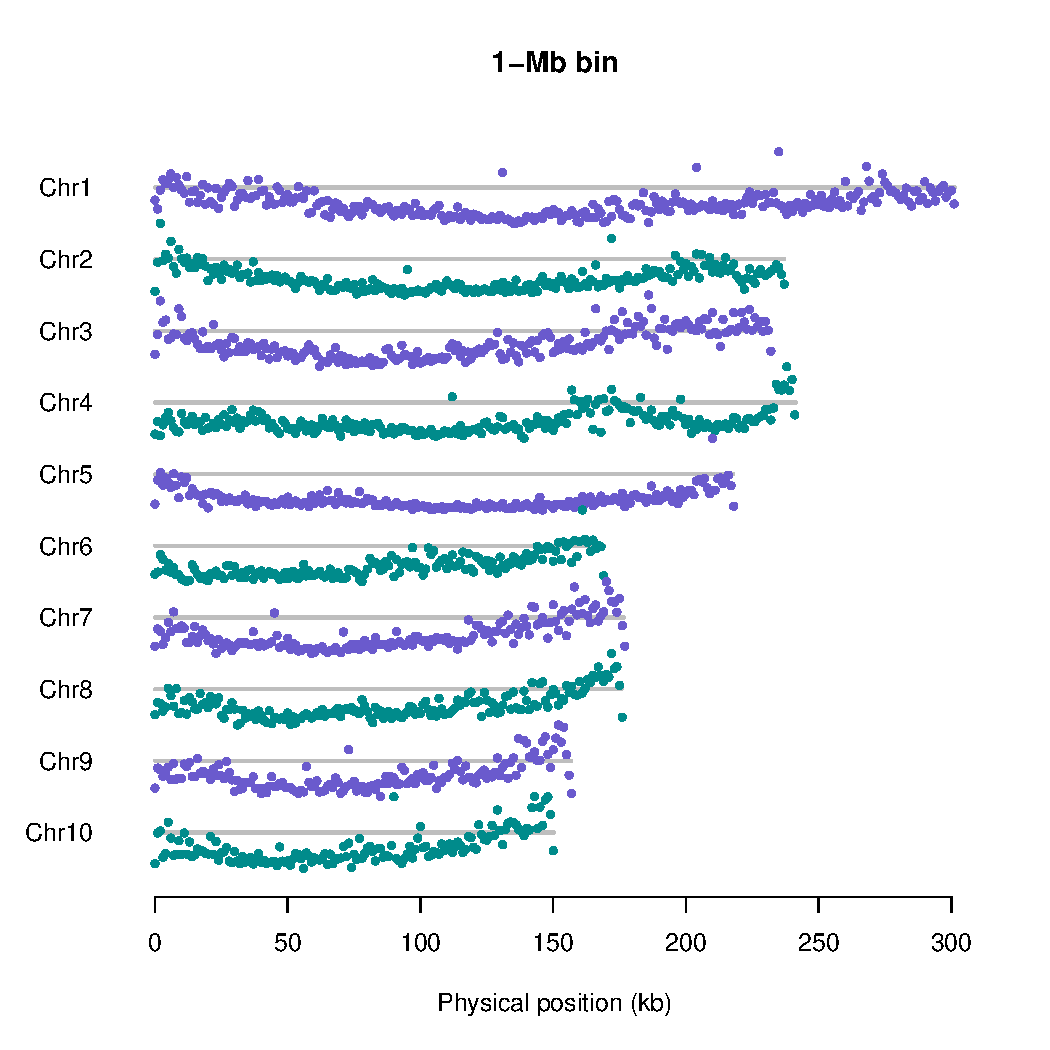
\includegraphics[width=\linewidth]{SFig_gerp_dis1m.pdf}
\caption{GERP score distribution across the genome. On the y-axis are the mean GERP scores in a 1-Mb bin region.}
\label{fig:dis1m}
\end{figure}

\begin{figure}[here]
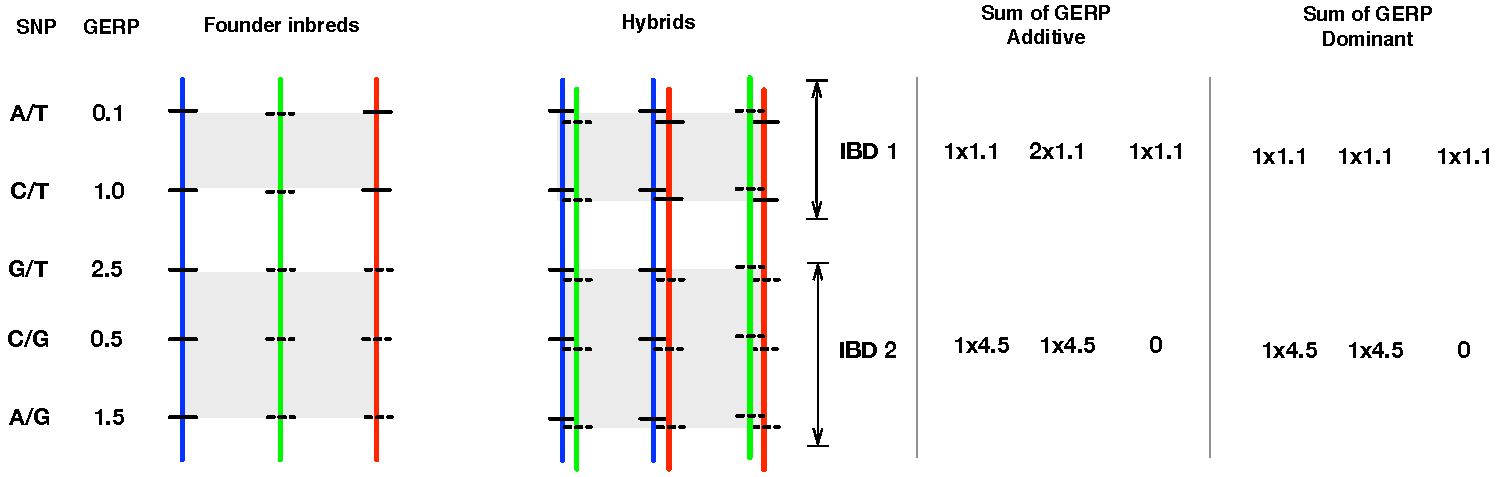
\includegraphics[width=0.9\textwidth]{SFig_gerpIBD.pdf}
\caption{
\textbf{Incoporation of conservation information into IBD blocks.}
Regions of the genome that are identical by descent (IBD) among the 12 inbreds were identified using Beagle \citep{Browning2009}.  The GERP scores of SNPs in an IBD block were summed under both additive and dominant models. Under the additive model, 2 x GERP score was assigned to genotypes homozygous for the non-reference allele, 1 x GERP score was assigned to heterozygotes, and 0 was assigned to the homozygous reference genotype. Under the dominant model, 1 x GERP score was assigned to both genotypes with a nonreference allle and 0 to the homozygous reference genotype.}
\label{fig:gerpibd}
\end{figure}

\begin{figure}[htbp]
\centering
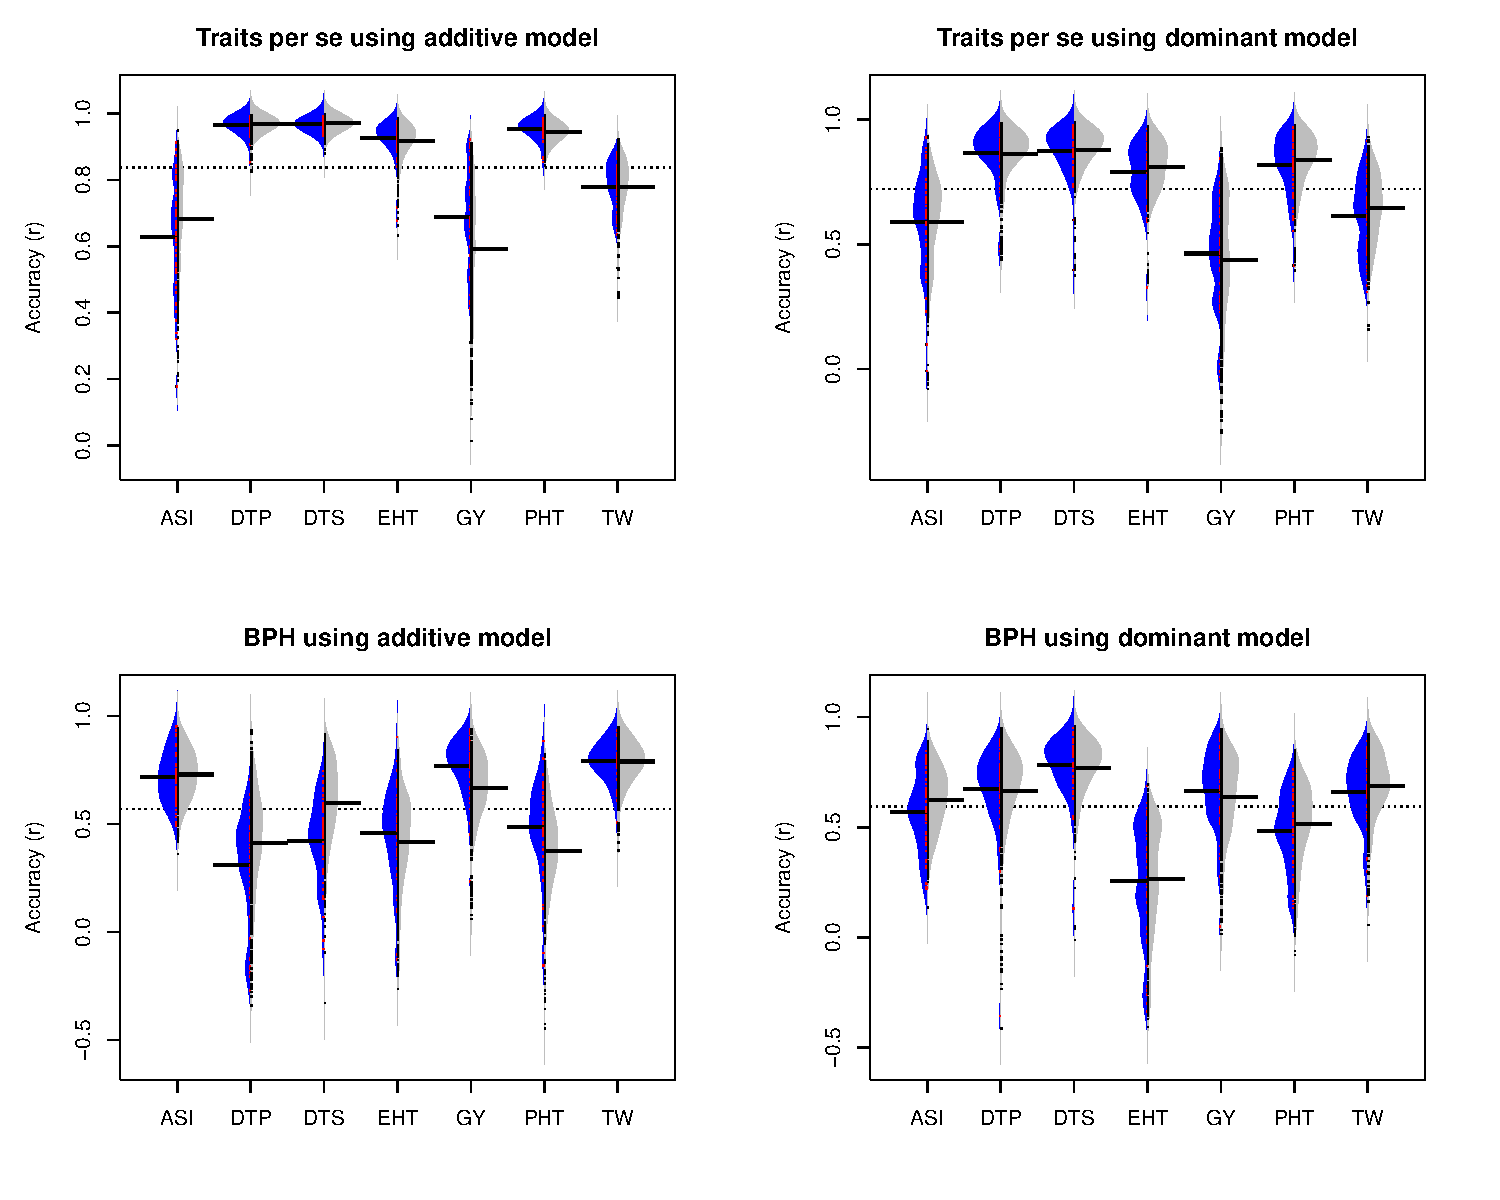
\includegraphics[width=\linewidth]{SFig_genicsnp.pdf}
\caption{Beanplots of cross-validation accuracies using genic SNPs. Cross-validation experiments were conducted using genic SNPs and circular shuffled data from the same set of the genic SNPs for traits \emph{per se} (\textbf{A, B}) and pHPH (\textbf{C, D}) under additive (\textbf{A, C}) and dominant (\textbf{B, D}) models. Accuaries from the real data were plotted on the left side of the bean (blue) and permutation results plotted on the right (grey). Horizotal bars on beans indicate mean accuracies. The grey dashed line indicates the overall average accuracy. Stars indicate significantly improved cross-validation accuracies.}
\label{fig:genicsnp}
\end{figure}

\end{document}